\documentclass{article}

\usepackage[a4paper, margin=1in]{geometry}
\usepackage{graphicx}
\usepackage{multicol}
\usepackage{listings}
\usepackage{xcolor}

\lstset{
  backgroundcolor=\color{black!5},
  frame=single,
  showstringspaces=false,
  numbers=left,
  numbersep=5pt,
  numberstyle=\tiny\color{black!70},
  basicstyle=\footnotesize\ttfamily,
  keywordstyle=\bfseries\color{green!60!black},
  commentstyle=\itshape\color{purple!80!black},
  identifierstyle=\color{blue!80!black},
  stringstyle=\color{orange!90!black},
  title=\lstname
}

\setlength\parindent{0pt}
\setlength\parskip{1em}

\title{USTH ICTM1 - Project S1 \\ \bigskip OpenGL}
\author{Tung \textsc{Nguyen} \and Agwu \textsc{Chinedu}}
\date{Supervisor: Dr. \textsc{Tran} Giang Son \\ \medskip
February 23, 2018}

\begin{document}

\maketitle

\textbf{OpenGL} - Open Graphics Library specifies a way to render graphics on the computer
screen. Provides a means for transferring data between CPU and GPU or directly to the GPU.

\begin{figure}[h]
\begin{center}
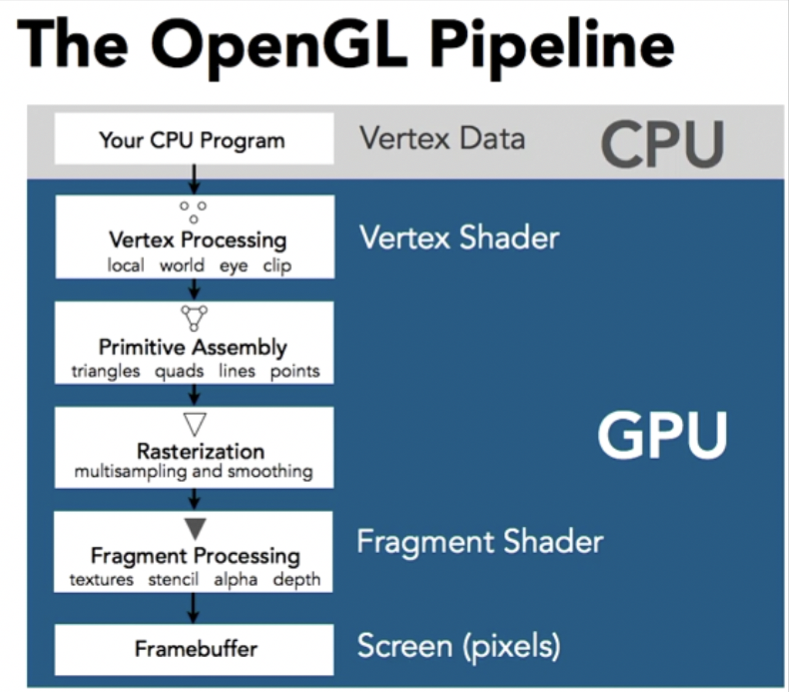
\includegraphics[width=0.8\textwidth]{pipeline}
\caption{OpenGL Pipeline Structure \footnotemark}
\end{center}
\end{figure}
\footnotetext{Lynda.com}

\textbf{GLSL} - OpenGL Shading Language is a language that works for several parts of the graphic card in the computer. We can write short GLSL programs, called SHADERS, that are executed on the GPU. \par

We need shaders so we can write different types of really nice features and possibilities, examples are writing: Shadows, Environment Mapping, Per-Pixel Lighting, Bump Mapping, Parallax Bump Mapping, HDR, ... \par

Two major types of shaders in GLSL:
\begin{itemize}
  \item \textbf{The Vertex Shader} simply tells the GPU where each vertex should be placed or rather the positions on the screen.
  \item \textbf{The Fragment Shader} runs once for every pixel that needs to get rasterized. It will mainly decide what colour to shade each pixel.
\end{itemize}

The Primitive or Triangle assembly connects all vertexes together as the programs specifies. \par

Rasterization in simple term means to drawn on the screen. \par

\textit{The below diagram shows more specific the process of working with shaders.}

\begin{figure}[h]
\begin{center}
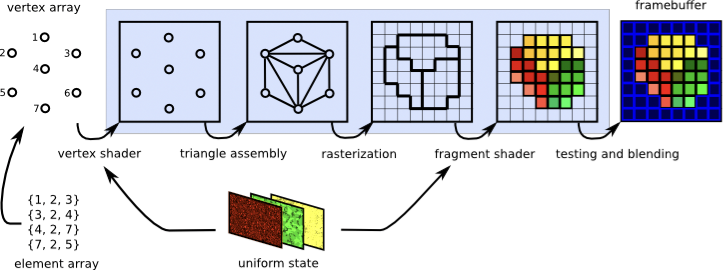
\includegraphics[width=0.9\textwidth]{detail-pipeline}
\caption{Detailed OpenGL Pipeline Structure \footnotemark}
\end{center}
\end{figure}
\footnotetext{https://www.enlightenment.org/playground/evas-gl.md}

\begin{multicols}{2}
\textbf{\textit{An OpenGL program example:}}
\lstinputlisting[language=C++]{example.cpp}

\columnbreak

\textbf{\textit{Output:}}
\begin{center}
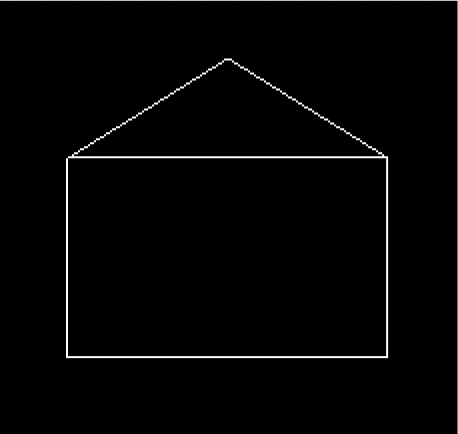
\includegraphics{example-output}
\end{center}
\end{multicols}

\end{document}